% $Id: introduction.tex 476 2019-01-18 14:13:50Z gsoyez $
%
% Introduction to jet physics, substructure and what is (and is not)
% covered in these lecture notes
% ------------------------------------------------------------------------
\chapter{Introduction and motivation}\label{chap:introduction}

The Large Hadron Collider (LHC) at CERN is the largest and most
sophisticated machine to study the elementary building blocks of
nature ever built.
%
At the LHC protons are brought into collision with a large
centre-of-mass energy --- 7~and 8~TeV for Run I (2010-13), 13~TeV for
Run~II (2015-18) and 14~TeV from Run III (starting in 2021) onwards
--- to resolve the smallest structures in a controlled and
reproducible environment. As protons are not elementary particles
themselves, but rather consist of quarks and gluons, their
interactions result in highly complex scattering processes, often with
final state populated with hundreds of particles, which are measured
via their interactions with particle detectors.

Jets are collimated sprays of hadrons, ubiquitous in collider
experiments, usually associated with the production of an elementary
particle that carries colour charge, e.g.\ quarks and gluons. Their
evolution is governed by the strong force, which within the Standard
Model of particle physics is described by Quantum Chromodynamics
(QCD).  The parton (\ie quark or gluon) that initiates a jet may
radiate further partons and produce a (collimated) shower of quarks
and gluons, a so-called parton shower, that eventually turn into the
hadrons ($\pi$, $K$, $p$, $n$,...) observed in the detector.  The vast
majority of LHC events (that one is interested in) contain jets. They
are the most frequently produced and most complex objects measured at
the LHC multipurpose experiments, ATLAS and CMS.

When protons collide inelastically with a large energy transfer
between them, one can formally isolate a hard process at the core of
the collision, which involves one highly-energetic parton from each of
the two protons. These two partons interact and produce a few
elementary particles, like two partons, a Higgs boson associated with
a gluon, a top--anti-top pair, new particles, ... Since the energy of
this hard process is large, typically between 100~GeV and several TeV,
there is a large gap between the incoming proton scale and the hard
process on one hand, and between the hard process and the hadron scale
on the other. This leaves a large phase-space for parton showers to
develop both in the initial and final state of the collision.
%
This picture is clearly a simplification because we can imagine that
secondary parton-parton interactions might take place. These
multi-parton interactions constitute what is usually referred to as
the \emph{Underlying Event}.
%
To complicate things further, the LHC does not collide individual
protons, but bunches of $\mathcal{O}(10^{11})$ protons. During one
bunch crossing it is very likely that several of the protons scatter
off each other. While only one proton pair might result in an event
interesting enough to trigger the storage of the event on tape, other
proton pairs typically interact to give rise to hadronic activity in
the detectors. This additional hadronic activity from multiple proton
interactions is called \emph{pileup}. On average, radiation from
pileup is much softer than the jets produced from the hard
interaction, but for jet (and jet substructure) studies it can have a
significant impact by distorting the kinematic relation of the jet
with the hard process.


In recent years the detailed study of the internal structure of jets
has gained a lot of attention.  At LHC collision energy electroweak
(EW) scale resonances, such as the top quark, W/Z bosons and the Higgs
boson, are frequently produced beyond threshold, i.e.\ their energy
(transverse momentum) can significantly exceed their mass.
%
Therefore, analyses and searching strategies developed for earlier
colliders, in which EW-scale particles were produced with small
velocity, have to be fundamentally reconsidered.
%
Because EW resonances decay dominantly into quarks, when they are
boosted, their
decay products can become collimated in the lab-frame and result in one large and massive jet, often referred to
as a fat jet. Initially such a configuration was considered
disadvantageous in separating processes of interest (\ie processes
which included EW resonances) from the large QCD backgrounds (where
jets are abundantly produced from high-energy quarks and
gluons).
%
However, with the popularisation of sequential jet clustering
algorithms retaining the full information of the jet's recombination
history, it transpired that one can use the internal structure of jets
to tell apart jets that were induced by a decaying boosted EW
resonance or by a QCD parton.
%
{\em This investigation of the internal structure of jets is what one
  refers to as jet substructure}.

While the first jet substructure methods have been put forward in the
1990s and early
2000s~\cite{Seymour:1991cb,Seymour:1993mx,Seymour:1994by,Butterworth:2002tt},
it was only in 2008, with the proposal to reconstruct the Higgs boson
in vector-boson associated production~\cite{Butterworth:2008iy}, that
the interest in understanding and utilising jet substructure surged
tremendously~\cite{Abdesselam:2010pt,Altheimer:2012mn,Altheimer:2013yza,Adams:2015hiv,Larkoski:2017jix,Asquith:2018igt}. If
the Higgs boson, being spin and colour-less, the perfect prototype of
a featureless resonance could be reconstructed, surely other
EW-scale resonances proposed in many extensions of the Standard Model could be
discovered as well. 
%
Furthermore, jet substructure can be exploited in searches of physics beyond the Standard Model (BSM) not necessarily restricted to the EW scale. 
%
For instance, in many such extensions TeV-scale resonances are
predicted which decay subsequently into EW particles, which could either be Standard Model or BSM resonances.
%
Because of the mass differences, these EW-particles are typically
boosted and their hadronic decay might be reconstructed as a fat jet.
%
Thus, scenarios where jet substructure methods can benefit searches
for BSM physics are rather frequent.

\begin{figure}
\begin{center}
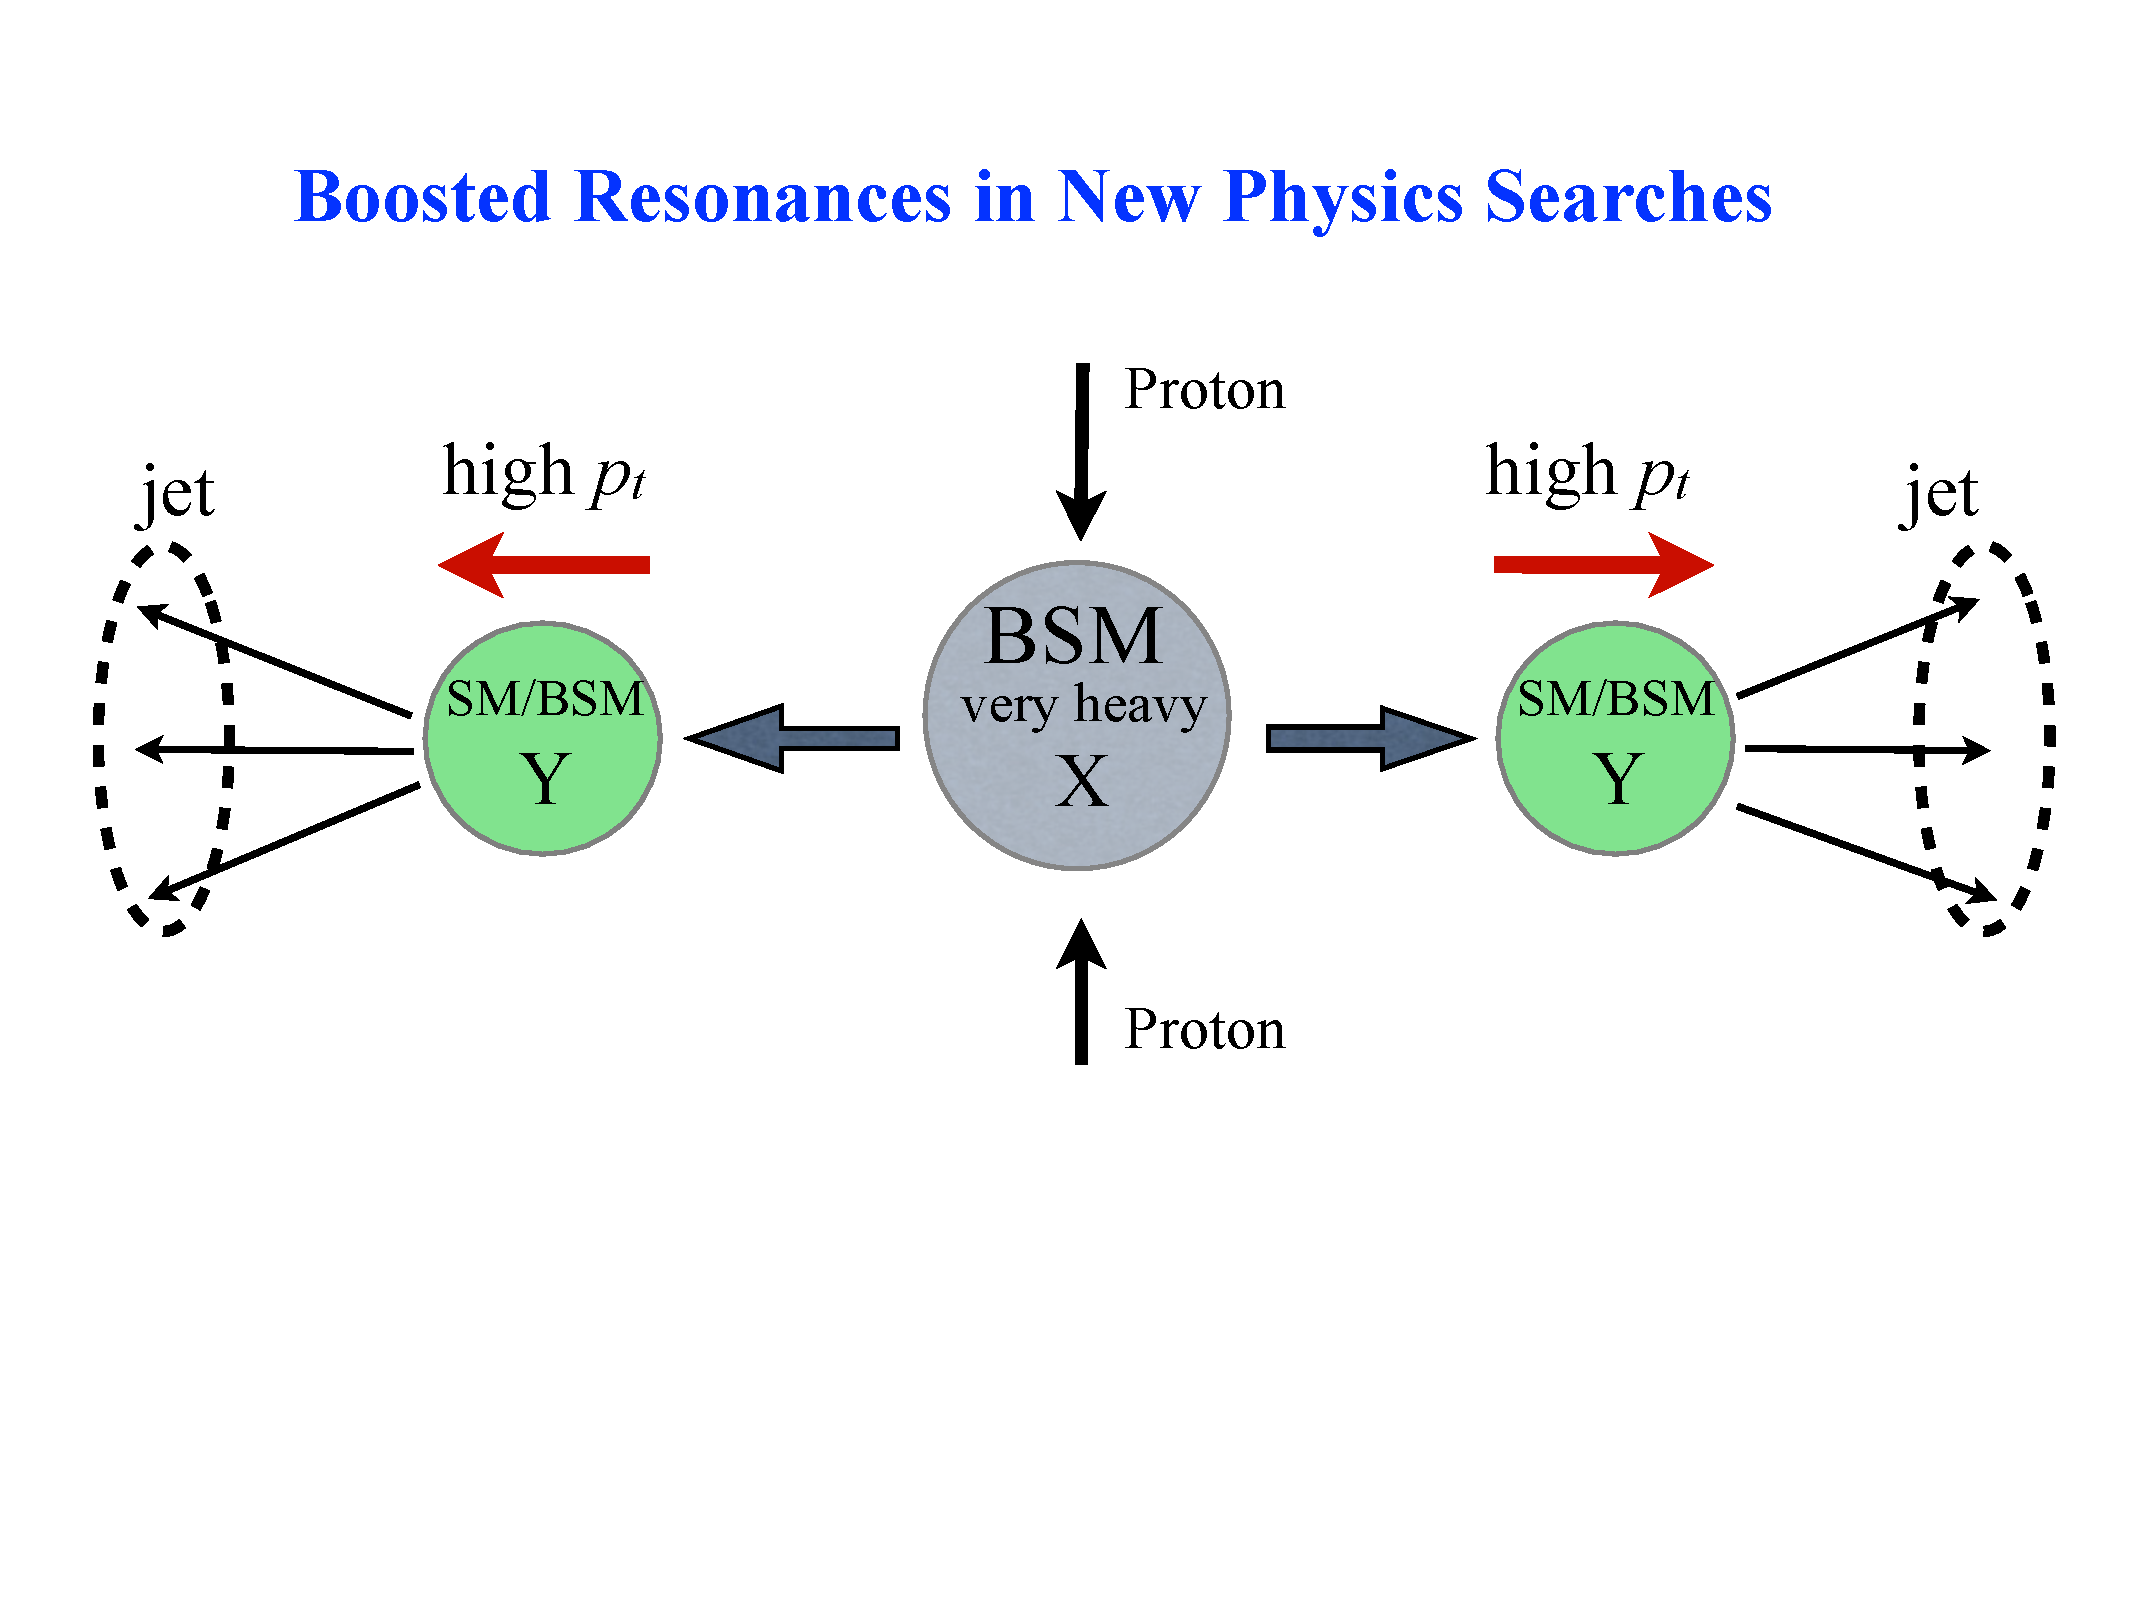
\includegraphics[width=0.9\textwidth]{figures/resonances}
\caption{Generic interaction sequence for the search of a very BSM
  resonance that decays into electroweak-scale particles that
  subsequently decay hadronically.}
\label{fig:resonance} 
\end{center}
\end{figure}
A typical situation of interest for BSM searches using jet
substructure is illustrated in Fig.~\ref{fig:resonance}. A heavy new
resonance X with a mass of $\mathcal{O}{(1)}$ TeV is produced in a
proton-proton collision. This heavy BSM resonance quickly decays into
lighter states Y --- \eg W/Z/H bosons or lighter BSM particles ---,
with a mass around the EW scale. Particles Y are
typically produced with large transverse momentum ($p_t$) because
their mass is much smaller than the mass of the decaying particle
X. Finally, if a particle Y decays hadronically, because of its
large boost, its decay product in the lab frame are collimated and
reconstructed into a jet. The aim of jet substructure is therefore to
distinguish a \emph{signal jet}, originated from a boosted massive
particles, such as Y, from \emph{background jets}, which typically are
QCD jets originated from quarks and gluons.


Consequently various ways of discriminating the sources of jets have
been devised, with the aim to classify a jet as of interest for a
specific search or measurement or not. Most methods to achieve this
classification task follow a two-step approach: firstly, the jet is
cleaned up ({\it groomed}), i.e.\ soft radiation which is unlikely to
come from the decaying resonance is removed, and, secondly, one
computes observables specifically designed to separate signal and
background jets based on the energy distribution amongst the remaining
jet constituents. Step two could be subdivided further into two
classes of classifiers: {\it jet-shape observables} and {\it
  prong-finders}. Jet-shape observables only consider the way the
energy is spatially distributed inside a jet, e.g.\ they do not take
into account the recombination history of the fat jet
itself. Prong-finders instead aim to construct hard subjets inside a
fat jet, i.e.\ isolated islands of energy inside the jet, and compare
properties of subjets, potentially including information on their
formation in the fat jet's recombination history.

Both jet shapes and prong finders aim to disentangle the different
topologies that characterise signal and background jets. For instance,
QCD jets are characterised by a hard core surrounded by soft/collinear
radiation, leading predominantly to jets with a one-prong
structure. EW bosons instead, such as W/Z and the Higgs, decays in a
quark-antiquark pair, which roughly share equal fractions of the heavy
particle momentum, leading to a two-prong structure. Finally, the top
quark preferentially decays into a bottom quark and a W boson, which
then decays in a pair of light quarks. Hence, top-initiated jets
features a three-pronged structure.
%
It has been shown that grooming techniques and jet substructure
observables are sensitive to different effects during the complex
evolution of a jet, hence the classification of jets benefits
from combining various of these techniques~\cite{Soper:2010xk,
  Adams:2015hiv}.\footnote{Finding hard subjets (the task of
  prong-finders) and removing soft contamination (the task of
  groomers) are similar in practice. This means that tools which do
  one, very often do the other as well.} Thus, by combining groomers
and different subjet observables, high-level tagging methods can be
constructed for the reconstruction of top quarks, W/Z and Higgs bosons
and new-physics resonances.

Nowadays, the application of jet substructure techniques has
considerably widen and goes well beyond the identification of massive
boosted particles.  A specific example particularly relevant for this
book is that because grooming techniques reduce an observable's
sensitivity to soft physics, comparisons between experimental data and
first-principle calculations are less affected by non-perturbative
contamination. Consequently, the catalogue of Standard Model
measurements with jet substructure techniques keeps
growing. Furthermore, jet substructure techniques have found
applications also in initially unexpected ways. For instance, it has
been realised that substructure variables can be used to probe the jet
interaction with the quark-gluon plasma in heavy-ion collisions,
providing new observables helping to improve our understanding of this
difficult question. Finally, particle physics in general, and jet
physics in particular, is enjoying a period of rapid development as
innovative ideas and techniques exploiting machine-learning are poured
into the field. Unfortunately, this topic goes beyond the scope of
this book and we refer the interested reader to the recent
review~\cite{Larkoski:2017jix}.

Although this book focuses on LHC physics, it is worth pointing out
that jet substructure techniques have also been used at other
colliders, such as the Tevatron or RHIC. Due to the lower collision
energy, the scope of substructure studies is more limited. We can
however point the readers to
Refs.~\cite{Almeida:2011ud,Altheimer:2012mn} for reviews of
substructure studies at the Tevatron and to Ref.~\cite{Kauder:2017mhg}
for an explicit measurement by the STAR collaboration at RHIC.
 
%\vspace{0.2 cm}

These lecture notes aim to provide an accessible entry --- at the
level of graduate students with some expertise in collider
phenomenology --- to the quickly growing field of jet substructure
physics. Due to the complexity of the internal structure of jets, this
topic connects to subtle experimental and quantum-field theoretical
questions. In order to make these notes as self-contained as possible,
the first four chapters will provide a broad introduction to jet
physics and related QCD ingredients. First, we will give a brief
introduction into QCD and its application to collider phenomenology in
Chapter~\ref{chap:qcd-colliders}, focusing on those aspects that are
needed the most in jet physics. Chapter~\ref{chap:jets-and-algs} will
introduce the basics of jet definition and jet algorithms, including
some of the experimental issues related to defining and measuring
jets.  In Chapter~\ref{chap:calculations-jets}, we will discuss in
some detail a key observable in jet physics, namely the jet invariant
mass. We will show how its theoretical description requires an
all-order perturbative approach and we will discuss various aspects of
this resummation.
%
We will dive into the topic of modern jet substructure in
Chapter~\ref{tools} where we will  first describe the main concepts and
ideas behind substructure tools and then try to give an comprehensive
list of the different approaches and tools which are currently
employed by the substructure community (theoretical and experimental).
%
Chapters~\ref{calculations-substructure-mass}-\ref{sec:curiosities}
explore our current first-principle understanding of jet
substructure with each chapter addressing a different application.
%
First, in Chapter~\ref{calculations-substructure-mass} we discuss
groomers which have been the first tools for which an analytic
understanding became available. In particular, we will go back to the
jet mass and we will study in detail how its distribution is modified
if grooming techniques are applied.  In the remaining chapters, we
will discuss more advanced topics such as quark/gluon discrimination
in Chapter~\ref{sec:calc-shapes-qg}, two-prong taggers in
Chapter~\ref{chap:calc-two-prongs} and, finally, Sudakov safety in
Chapter~\ref{sec:curiosities}.
%
Finally, in the last part of this book, we will discuss the current
status of searches and measurements using jet substructure in
Chapter~\ref{searches-measurements}.

%\vspace{0.2 cm}


A large part of these lecture notes will focus on our current
first-principle understanding of jet substructure in QCD.
%
The key observation to keep in mind in this context is the fact that
substructure techniques are primarily dealing with boosted jets, for
which the transverse momentum, $p_t$, is much larger than the mass,
$m$.
%
From a perturbative QCD viewpoint, this means that powers of the
strong coupling will be accompanied with large logarithms of $p_t/m$,
a common feature of QCD whenever we have two largely disparate scales.
%
For these situations, a fixed-order perturbative approach is not
suited and one should instead use all-order, {\em resummed},
calculations which focus on including the dominant
logarithmically-enhanced contributions at all orders in the strong
coupling.
%
Chapter~\ref{chap:calculations-jets} will present a basic
introduction to resummation taking the calculation of the jet mass as
a practical example.


There exist different approaches on how to tackle this type of
calculations. On the one hand, one could analyse the structure of
matrix elements for an arbitrary number of quark and gluon emissions
in the soft/collinear limit and from that derive the all-order
behaviour of the distribution of interest. In this context, the
coherent branching algorithm~\cite{Catani:1990rr,Catani:1992ua}
deserves a special mention because not only it is the basis of
angular-ordered parton showers, but it also constitutes the foundation
of many resummed calculations (for a review see
e.g.~\cite{Luisoni:2015xha}). Other approaches to all-order
resummation instead take a more formal viewpoint and try to establish
a factorisation theorem for the observable at hand, therefore
separating out the contribution from hard, soft and collinear
modes. This point of view is for instance, the one taken when
calculations are performed in Soft-Collinear Effective Theory
(SCET). For a pedagogical introduction to SCET, we recommend
Ref.~\cite{Becher:2014oda}.

In this book, we will use the former approach, but we will try to
point out the relevant literature for SCET-based calculations too.
%
That said, our aim is not to present a rigorous and formal proof of
resummed calculations, but rather to lay out the essential ingredients
that go into these theoretical predictions, while keeping the
discussion at a level which we think it is understandable for readers
with both theoretical and experimental backgrounds.
%
In particular, even though
Chapters~\ref{calculations-substructure-mass}-\ref{sec:curiosities}
start with (sometimes heavy) analytic QCD calculations, we will always
come back to comparisons between these analytic calculations and Monte
Carlo simulations in the end.
%
This will allow us to discuss the main physical features of the
observed distributions and how they emerge from the analytic
understanding. It will also allow us to discuss how the analytic
results obtained in perturbative QCD are affected by non-perturbative
corrections.


%% GS helper for auctex
%%% Local Variables:
%%% mode: latex
%%% TeX-master: "notes"
%%% End:

%  LocalWords:  EW BSM SCET
